\section{Auswertung}
\label{sec:Auswertung}
Die Werte für die Wellenlänge $\lambda$ des Lasers, sowie der Abstand $L$ vom optischen Element zum
Detektor betragen:
\begin{align*}
  \lambda=&\SI{635}{\nm}\\
  L=&\SI{1,085}{\m}.
\end{align*}

Für den Dunkelstrom wurden
\begin{equation*}
   I_{\text{Dunkel}}=\SI{0.1}{\nA}
\end{equation*}
gemessen. Außerdem kann für den Winkel $\phi$ mit Hilfe der Kleinwinkelnäherung
\begin{equation}
  \phi= \frac{x-x_{0}}{L}
\end{equation}
angenommen werden.

Die Messwerte für den ersten Doppelspant sind in Tabelle \ref{tab:tabelle1} zu sehen.
Mit Hilfe einer Ausgleichsfunktion werden die Werte für die Spaltbreite $b$, den
Spaltabstand $s$, die Amplitude $i_0$ und die Verschiebung des Maximuns vom Nullpunkt $x_{0}$ bestimmt.
Diese Ausgleichsfunktion wird nach Gleichung \ref{eqn:doppelinf} berechnet und ist in
Abbildung \ref{fig:plot1} zu sehen. Da die Messwerte nicht ganz symmetrisch sind werden
die rechte und linke Seite der Messwerte für die Ausgleichsgerade getrennt betrachtet.
Außerdem werden dem Programm Startwerte vorgegeben, dafür wurde $i_0$ aus \ref{tab:tabelle1}
abgelesen und für $b$ und $s$ wurden die Herstellerangaben als Startwerte gewält.
Für den ersten Spalt sind
\begin{align*}
  b=\SI{0,15}{\mm} &\;\;\;\;\;\;\;\;\;\; s=\SI{1}{\mm}
\end{align*}
vom Hersteller angegeben.

\begin{table}[H]
  \centering
  \caption{Messwerte der Wärmepumpe}
  \label{tab:tabe1}
    \begin{tabular}{S S S S S S}
    \toprule
    $ t  \: / \si{\second} $ & $ p_a \: / \si{\bar} $ & $ p_b \: / \si{\bar} $ &
    $ T_1 \: / \si{\kelvin} $ & $ T_2 \: / \si{\kelvin} $ & $ P \: / \: \si{\watt} $\\
    \midrule
    0 & 5.0 & 5.0 & 293.65 & 293.65 & 0 \\
    60 & 4.7 & 6.0 & 294.15 & 293.55 & 115 \\
    120 & 4.4 & 6.4 & 295.15 & 293.15 & 118 \\
    180 & 4.5 & 6.9 & 296.35 & 291.95 & 122 \\
    240 & 4.6 & 7.0 & 297.55 & 290.95 & 125 \\
    300 & 4.6 & 7.0 & 298.85 & 289.95 & 125 \\
    360 & 4.5 & 7.2 & 300.05 & 289.15 & 123 \\
    420 & 4.4 & 7.4 & 301.15 & 288.45 & 123 \\
    480 & 4.3 & 7.8 & 302.35 & 287.65 & 122 \\
    540 & 4.2 & 8.0 & 303.55 & 286.95 & 122 \\
    600 & 4.2 & 8.1 & 304.65 & 286.25 & 121 \\
    660 & 4.1 & 8.3 & 305.75 & 285.55 & 121 \\
    720 & 4.0 & 8.5 & 306.75 & 284.95 & 121 \\
    780 & 4.0 & 8.8 & 307.75 & 284.35 & 121 \\
    840 & 3.9 & 9.0 & 308.75 & 283.75 & 121 \\
    900 & 3.8 & 9.1 & 309.65 & 283.15 & 121 \\
    960 & 3.8 & 9.2 & 310.55 & 282.55 & 122 \\
    1020 & 3.8 & 9.5 & 311.45 & 282.05 & 122 \\
    1080 & 3.7 & 9.8 & 312.25 & 281.55 & 122 \\
    1140 & 3.7 & 10.0 & 313.05 & 281.15 & 122 \\
    1200 & 3.7 & 10.0 & 313.9 & 280.65 & 122 \\
    1260 & 3.6 & 10.2 & 314.65 & 280.25 & 123 \\
    1320 & 3.6 & 10.3 & 315.35 & 279.85 & 123 \\
    1380 & 3.6 & 10.6 & 316.15 & 279.45 & 124 \\
    1440 & 3.6 & 10.8 & 316.85 & 279.15 & 124 \\
    1500 & 3.6 & 11.0 & 317.55 & 278.75 & 124 \\
    1560 & 3.6 & 11.1 & 318.25 & 278.55 & 124 \\
    1620 & 3.6 & 11.2 & 318.95 & 278.25 & 125 \\
    1680 & 3.5 & 11.4 & 319.55 & 277.95 & 125 \\
    1740 & 3.5 & 11.5 & 320.15 & 277.65 & 125 \\
    1800 & 3.5 & 11.7 & 320.75 & 277.45 & 125 \\
    1860 & 3.5 & 11.9 & 321.35 & 277.25 & 125 \\
    1920 & 3.5 & 12.0 & 321.95 & 277.05 & 125 \\
    1980 & 3.5 & 12.1 & 322.45 & 276.95 & 125 \\








      \bottomrule
    \end{tabular}
\end{table}

\begin{figure}
  \centering
  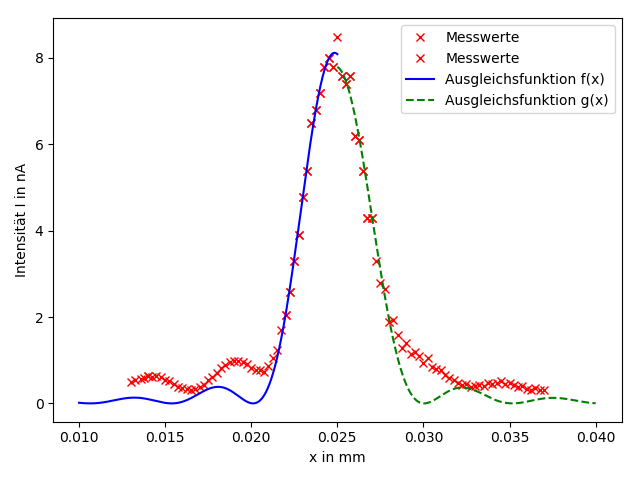
\includegraphics[height=7cm]{Figure_1.png}
  \caption{Messwerte und Ausgleichsfunktion für den ersten Doppelspalt.}
  \label{fig:plot1}
\end{figure}

Die Regression ergibt für den erten Spalt folgende Werte:
\begin{align*}
  I =& \SI{8.1(2)}{\nA}\\
  B =& \SI{1.77(8)e-4}{\mm}\\
  S =& \SI{24.84(4)}{\mm}\\
  M =& \SI{0.13(1)}{\mm}\\
  i =& \SI{7.8(2)}{\nA}\\
  b =& \SI{9(198564)e-7}{\mm}\\
  s =& \SI{24.9(4)}{\mm}\\
  m =& \SI{0.1(34)}{\mm}
\end{align*}

Dabei wurden die Parameter der linken Seite mit Großbuchstaben, die Parameter der rechten Seite
mit Kleinbuchstaben bezeichnet. Da die Messwerte wie in \ref{fig:plot1} zu sehen auf der rechten
Seite nicht zum zu erwartenden Interferenzbild passen sind die Parameter dmentsprechend ungenau und
zum Teil mit großen Fehlern belastet. Daher werden im Folgenden die Werte für
$b$ und $m$ nicht beachtet.

Um die Messwerte mit den Herstellerangaben zu vergleichen wird die Abweichung nach folgender
Formel berechnet:
\begin{equation}
  \text{Abweichung}=\frac{\text{Messwert}-\text{Herstellerangabe}}{\text{Herstellerangabe}}\cdot100
\end{equation}
Daraus ergibt sich, dass die Spaltbreite $b$ um 18\% abweicht
und der Spaltabstand $s$ um 2387\%.
Um die Abweichung der Nulllinie zu bestimmen wird
der Winkel $\phi$ nach $\phi=\frac{x-x_{0}}{L}$ berechnet. Theoretisch liegt die
Nulllinie bei $\Delta \phi=0\;\text{rad} $. Es ergibt sich
\begin{equation*}
  \Delta \phi =\SI{0.0228(9)}\; \text{rad}.
\end{equation*}\\

Für den zweiten Doppelspalt wird anaglog vorgegeangen, die Messwerte sind in Tabelle
\ref{tab:tabelle2} zu finden und die Ausgleichsfunktion in Abbildung \ref{fig:plot2}.
Auch hier wird die Ausgleichsunktion aufgeteilt, die Parameter der linken Seite weden mit
Großbuchstaben beschieben und die der rechten Seite mit Kleinbuchstaben. Außerdem wurden erneut die Herstellerangaben
als Startwerte vorgegeben und $I_0$ aus Tabelle \ref{tab:tabelle2} abgelesen.
Für diesen Doppelspalt wurden vom Hersteller
\begin{align*}
  b=\SI{0,1}{\mm}  &\;\;\;\;\;\;\;\;\;\; s=\SI{0,4}{\mm}
\end{align*}
angegeben.

\begin{table}[H]
  \centering
  \caption{Wertetabelle für $\alpha$ und $C_V$.}
  \label{tab:tab2}
    \begin{tabular}{S S S S S}
    \toprule
    $ T\: \text{in}\: \si{\K} $ & $ {\alpha \cdot 10^{-6} \: \text{in}\: \si {\per\K}} $ &
    $ C_V \: \text{in}\: \si{\J\per\K\mol} $\\
    \midrule %Cv, a *10-6, Cv
    %0 & 1 & 1\\
    88.60\pm0.24 & 9.56\pm0.06 & 14.17\pm8.13  \\ %&3.6 & 318.97\pm0.85\\
    93.81\pm0.24 & 10.10\pm0.06 & 17.58\pm10.03 \\ %& 4.7 & 440.90\pm1.11\\
    99.74\pm0.24 & 10.66\pm0.05 & 15.52\pm8.84 \\ %& 5.1 & 508.68\pm1.21\\
    104.74\pm0.24 & 11.07\pm0.05 & 18.44\pm10.52 \\ %& 4.6 & 481.79\pm1.09\\
    110.94\pm0.24 &  11.54\pm0.05 & 14.86\pm8.45 \\ %& 5.3 & 587.97\pm1.27\\
    115.96\pm0.24 & 11.89\pm0.05 & 18.49\pm10.52 \\ %& 4.6 & 533.41\pm1.10\\
    121.47\pm0.24 &  12.22\pm0.05 & 16.83\pm9.57 \\ %& 4.9 & 595.21\pm1.17\\
    126.99\pm0.24 & 12.53\pm0.04 & 16.79\pm9.54 \\ %& 4.9 & 622.29\pm1.18\\
    131.58\pm0.24 & 12.77\pm0.04 & 20.42\pm11.62 \\ %& 4.2 & 552.62\pm1.01\\
    136.65\pm0.24 & 13.02\pm0.04 & 18.40\pm10.47 \\ %& 4.6 & 628.57\pm1.11\\
    141.49\pm0.24 & 13.24\pm0.04 & 19.28\pm10.97 \\ %& 4.4 & 622.54\pm1.07\\
    146.34\pm0.24 & 13.44\pm0.04 & 19.24\pm10.95 \\ %& 4.4 & 643.88\pm1.07\\
    150.95\pm0.24 & 13.62\pm0.04 & 20.22\pm11.52 \\ %& 4.3 & 649.11\pm1.05\\
    155.34\pm0.24 & 13.79\pm0.04 & 21.31\pm12.14 \\ %& 4.1 & 636.88\pm0.98\\
    159.97\pm0.24 & 13.95\pm0.04 & 20.12\pm11.47 \\ %& 4.3 & 687.89\pm1.05\\
    164.62\pm0.24 & 14.10\pm0.04 & 20.18\pm11.51 \\ %& 4.3 & 707.87\pm1.06\\
    168.79\pm0.25 & 14.23\pm0.04 & 22.54\pm12.86 \\ %& 3.9 & 658.27\pm0.95\\
    173.45\pm0.25 &  14.37\pm0.04 & 20.08\pm11.46 \\ %& 4.3 & 745.84\pm1.06\\
    178.13\pm0.25 &  14.50\pm0.04 & 20.04\pm11.44 \\ %& 4.3 & 765.94\pm1.06\\
    182.56\pm0.25 &  14.62\pm0.04 & 21.11\pm12.06\\
    192.70\pm0.25 &  14.87\pm0.04 & 18.41\pm10.47\\
    200.15\pm0.25 &  15.04\pm0.04 & 25.19\pm14.28\\
    208.87\pm0.25 &  15.23\pm0.04 & 21.43\pm12.18\\
    217.12\pm0.25 &  15.38\pm0.04 & 22.65\pm12.88\\
    225.15\pm0.25 &  15.53\pm0.03 & 23.27\pm13.24\\
    232.70\pm0.25 &  15.70\pm0.03 & 24.75\pm14.08\\
    240.53\pm0.25 &  15.74\pm0.03 & 23.84\pm13.58\\
    248.39\pm0.25 &  15.89\pm0.03 & 23.74\pm13.53& \\
    256.01\pm0.25 &  15.97\pm0.03 & 24.46\pm13.94 \\
    263.41\pm0.26 &  16.01\pm0.03 & 25.22\pm14.38 \\
    271.08\pm0.26 &  16.18\pm0.03 & 24.26\pm13.86 \\
    278.52\pm0.26 &  16.27\pm0.03 & 25.03\pm14.29&\\
    285.98\pm0.26 &  16.35\pm0.03 & 24.92\pm14.25 \\
    293.21\pm0.26 &  16.42\pm0.03 & 25.74\pm14.72 \\
    300.98\pm0.26 &  16.50\pm0.03 & 23.87\pm13.68 \\
    308.51\pm0.26 &  16.57\pm0.03 & 24.63\pm14.12\\



      \bottomrule
    \end{tabular}
\end{table}

\begin{figure}
  \centering
  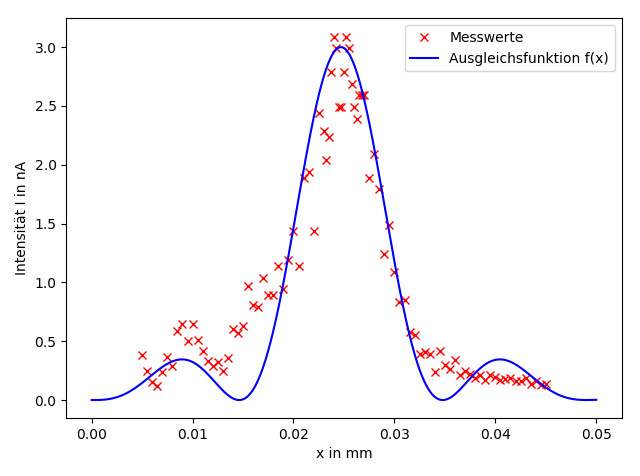
\includegraphics[height=7cm]{Figure_2.png}
  \caption{Ausgleichsfunktion und Messwerte des zweiten Doppelspaltes.}
  \label{fig:plot2}
\end{figure}

Hier ergibt die Regression:
\begin{align*}
 I =& \SI{3.42(27)}{\nA}\\
 B =& \SI{0.44(4)}{\mm}\\
 S =& \SI{25.54(0)}{\mm}\\
 M =& \SI{3.76(14)}{\mm}\\
 i =& \SI{3.7(3)}{\nA}\\
 b =& \SI{0.46(4)}{\mm}\\
 s =& \SI{25.4(0)}{\mm}\\
 m =& \SI{0.05(1)}{\mm}
\end{align*}

Die Abweichungen von den Herstellerangaben berechnen sich analog zum
ersten Doppelspalt, es ergibt sich für den Spaltabstand $s$ eine Abweichung von
6267.5\% und für die Spaltbreite eine Abweichung von 350\%. Für den Winkel der
Nulllinie ergibt sich:
\begin{equation}
  \Delta \phi =\SI{0.021(0)}\; \text{rad}.
\end{equation}

Für die Ausgleichfunktion in Abblildung \ref{fig:plot3} des Einzelspaltes
wird Gleichung \ref{eqn:einzel1} verwendet.
Die dazugehörigen Messwerte stehen in Tabelle \ref{tab:tabelle3}.
Wie zuvor auch wird die Ausgleichsfunktion wieder aufgespalten, Großbuchstaben
beschreiben die rechte Seite, Kleinbuchstaben die linke Seite.
Vom Hersteller wird hier die Spaltbreite mit $b=\SI{0,15}{\mm}$ angegeben.

\begin{table}
  \centering
  \caption{Messwerte für den ersten Doppelspalt.}
   \begin{tabular}{S S| S S | S S}
    \toprule
    $x/\; \si{\mm}$& $A/\;\si{\nA}$ &
    $x/\; \si{\mm}$& $A/\;\si{\nA}$ &
    $x/\; \si{\mm}$& $A/\;\si{\nA}$ \\
    \midrule

    15.0& 4.6& 23.0& 25.0& 29.5& 6.0\\
    15.5& 4.2& 23.5& 30.0& 30.0& 5.3\\
    16.0& 4.0& 24.0& 35.0& 30.5& 4.9\\
    16.5& 4.0& 24.25& 36.0& 31.0& 4.7\\
    17.0& 4.4& 24.5& 37.0& 31.5& 4.4\\
    17.5& 5.5& 24.75& 38.0& 32.0& 4.2\\
    18.0& 6.6& 25.00& 37.0& 32.5& 3.8\\
    18.5& 7.7& 25.25& 36.0& 33.0& 3.6\\
    19.0& 8.2& 25.5& 36.0& 33.5& 3.2\\
    19.5& 8.4& 26.0& 33.0& 34.0& 3.2\\
    20.0& 8.4& 26.5& 28.5& 34.5& 3.2\\
    20.25& 8.4& 27.0& 23.0& 35.0& 3.3\\
    20.5& 8,7& 27.5& 18.0& 35.5& 3.4\\
    21.0& 9.8& 28.0& 13.5& 36.0& 3.5\\
    21.5& 12.0& 28.5& 10.0\\
    22.0& 15.0& 29.0& 7.8\\
    22.5& 20.0& 29.25& 6.7\\


   \bottomrule
  \end{tabular}
  \label{tab:tabelle3}
\end{table}

\begin{figure}
  \centering
  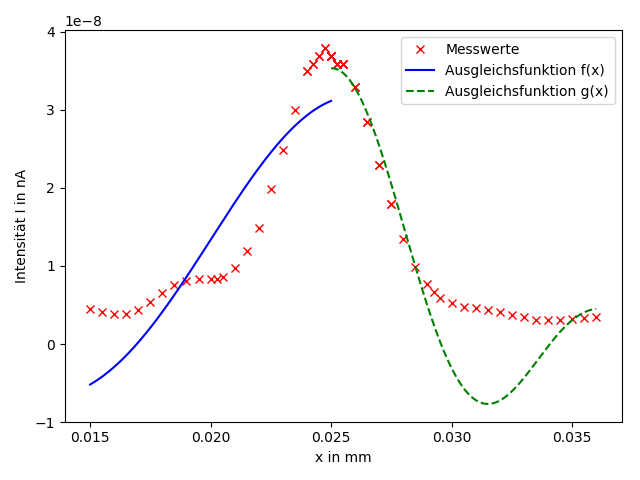
\includegraphics[height=7cm]{Figure_4.png}
  \caption{Ausgleichsfunktion und Messwerte des Einzelspaltes.}
  \label{fig:plot3}
\end{figure}

Die Regression ergibt für den Einzelspalt diese Werte:
\begin{align*}
  i =& \SI{5(1)}{\nA}\\
  b =& \SI{0.08(1)}{\mm}\\
  m =& \SI{26(1)}{\mm}\\
  I =& \SI{5.5(2)}{\nA}\\
  B =& \SI{0.08(1)}{\mm}\\
  M =& \SI{26(1)}{\mm}
\end{align*}
Hier ist zu beachten, dass der Wert des Maximums aus der Ausgleichsrechnung ausgenommen
wurde, da sich ansonsten kein numerisch zu verarbeitender Wert ergibt.
Hier beträgt die Abweichung der Spaltbreite -56.66\%.
Die Abweichung der Nulllinie wird äquivalent wie beim Doppelspalt berechnet.
Es ergibt sich
\begin{equation*}
  \Delta \phi= \SI{0.0005(9)}\; \text{rad}.
\end{equation*}
%0.006+/-0.028
